%  LaTeX support: latex@mdpi.com
%  For support, please attach all files needed for compiling as well as the log file, and specify your operating system, LaTeX version, and LaTeX editor.

%=================================================================
\documentclass[remotesensing,article,submit,pdftex,moreauthors]{Definitions/mdpi}

%=================================================================
% MDPI internal commands - do not modify
\firstpage{1}
\makeatletter
\setcounter{page}{\@firstpage}
\makeatother
\pubvolume{1}
\issuenum{1}
\articlenumber{0}
\pubyear{2024}
\copyrightyear{2024}
%\externaleditor{Academic Editor: Firstname Lastname}
\datereceived{ }
\daterevised{ } % Comment out if no revised date
\dateaccepted{ }
\datepublished{ }
%\datecorrected{} % For corrected papers: "Corrected: XXX" date in the original paper.
%\dateretracted{} % For corrected papers: "Retracted: XXX" date in the original paper.
\hreflink{https://doi.org/} % If needed use \linebreak
%\doinum{}
%\pdfoutput=1 % Uncommented for upload to arXiv.org
%\CorrStatement{yes}  % For updates


%=================================================================
% Add packages and commands here. The following packages are loaded in our class file: fontenc, inputenc, calc, indentfirst, fancyhdr, graphicx, epstopdf, lastpage, ifthen, float, amsmath, amssymb, lineno, setspace, enumitem, mathpazo, booktabs, titlesec, etoolbox, tabto, xcolor, colortbl, soul, multirow, microtype, tikz, totcount, changepage, attrib, upgreek, array, tabularx, pbox, ragged2e, tocloft, marginnote, marginfix, enotez, amsthm, natbib, hyperref, cleveref, scrextend, url, geometry, newfloat, caption, draftwatermark, seqsplit
% cleveref: load \crefname definitions after \begin{document}

%=================================================================
% Please use the following mathematics environments: Theorem, Lemma, Corollary, Proposition, Characterization, Property, Problem, Example, ExamplesandDefinitions, Hypothesis, Remark, Definition, Notation, Assumption
%% For proofs, please use the proof environment (the amsthm package is loaded by the MDPI class).

%=================================================================
% Full title of the paper (Capitalized)
\Title{Robot Team III: Scotty Strikes Back}

% MDPI internal command: Title for citation in the left column
\TitleCitation{Title}

% Author Orchid ID: enter ID or remove command
\newcommand{\orcidauthorA}{0000-0002-5910-0183} % John
\newcommand{\orcidauthorB}{0000-0003-2688-648X} % Lakitha
\newcommand{\orcidauthorC}{0000-0002-9841-6703} % Shawhin
\newcommand{\orcidauthorD}{0000-0003-2657-3416} % Prabuddha
\newcommand{\orcidauthorE}{0000-0003-4265-9543} % David
\newcommand{\orcidauthorF}{0000-0003-0667-2345} % Ash
\newcommand{\orcidauthorG}{0000-0002-0126-218X} % Adam
% \newcommand{\orcidauthorH}{} % Gokul

% Authors, for the paper (add full first names)
\Author{John Waczak \orcidA{}, Adam Aker \orcidG{}, Lakitha O. H. Wijeratne \orcidB{}, Shawhin Talebi \orcidC{}, Ashen Fernando \orcidF{}, Prabuddha M. H. Dewage \orcidD{}, Mazhar Iqbal, Matthew Lary, David Schaefer, Gokul Balagopal, and David J. Lary *\orcidE{}}

%\longauthorlist{yes}

% MDPI internal command: Authors, for metadata in PDF
\AuthorNames{John Waczak, Adam Aker, Lakitha O. H. Wijeratne, Shawhin Talebi, Bharana Fernando, Prabuddha Hathurusinghe, Mazhar Iqbal, Matthew Lary, David Schaefer, Gokul Balagopal, and David J. Lary}

% MDPI internal command: Authors, for citation in the left column
 \AuthorCitation{Waczak, J.; Aker, A.; Wijeratne, L.O.H.; Talebi, S.; Fernando, B.; Hathurusinghe, P.; Iqbal, M.; Lary, M.; Schaefer, Balagopal, G.; D.; Lary, D.J.}
% If this is a Chicago style journal: Lastname, Firstname, Firstname Lastname, and Firstname Lastname.

% Affiliations / Addresses (Add [1] after \address if there is only one affiliation.)
\address[1]{%
Hanson Center for Space Sciences, University of Texas at Dallas, Richardson, TX 75080, USA;  john.waczak@utdallas.edu (J.W.); adam.aker@utdallas.edu (A.A.); lhw150030@utdallas.edu (L.O.H.W.); shawhintalebi@gmail.com (S.T.); ashen.fernando@utdallas.edu  (B.F.); pxh180012@utdallas.edu (P.M.H.D.); mazhar.iqbal@utdallas.edu (M.I.); MDL210001@utdallas.edu (M.L.); captdaveschaefer@gmail.com (D.S.); gokul.balagopal@utdallas.edu (G.B.);}

% Contact information of the corresponding author
\corres{Correspondence: david.lary@utdallas.edu} %; Tel.: (optional; include country code; if there are multiple corresponding authors, add author initials) +xx-xxxx-xxx-xxxx (F.L.)}


% Abstract (Do not insert blank lines, i.e. \\) 
\abstract{
Unmanned Aerial Vehicles (UAVs) equipped with hyperspectral imagers have emerged as an essential technology for the characterization of inland water bodies. The high spectral and spatial resolutions of these systems enable the retrieval of a plethora of optically-active water quality parameters via band ratio algorithms and machine learning methods. However, fitting and validating these models requires access to sufficient quantities of in situ reference data which are time-consuming and expensive to obtain. In this study, we demonstrate how the Generative Topographic Mapping (GTM), a Bayesian realisation of the Self Organizing Map (SOM), enables highly-detailed unsupervised classification and nonlinear endmember extraction of UAV acquired hyperspectral imagery. Specifically, the topographic relationship between classes maintained by the GTM presents an attractive alternative to other unsupervised approaches which do not provide a notion of similarity between learned classes. Using data collected across a North Texas pond, we apply the GTM to create a detailed map segmenting the area into distinct regions of interest. Further, by interpreting the learned classes as distinct endmembers, the GTM can be used to rapidly identify and map unique water constituents. We demonstrate this capability by using the GTM to map algal abundance as well as the dispersion of a rhodamine dye tracer released into the water.
}

% Keywords
\keyword{Hyperspectral Imaging; Remote Sensing; Unsupervised Classification; Endmember Extraction, Spectral Unmixing} 


%%%%%%%%%%%%%%%%%%%%%%%%%%%%%%%%%%%%%%%%%%
\begin{document}

%%%%%%%%%%%%%%%%%%%%%%%%%%%%%%%%%%%%%%%%%%
\section{Introduction}


%%%%%%%%%%%%%%%%%%%%%%%%%%%%%%%%%%%%%%%%%%
\section{Materials and Methods}


\begin{figure}[t]
%\begin{adjustwidth}{-\extralength}{0cm}
\centering
%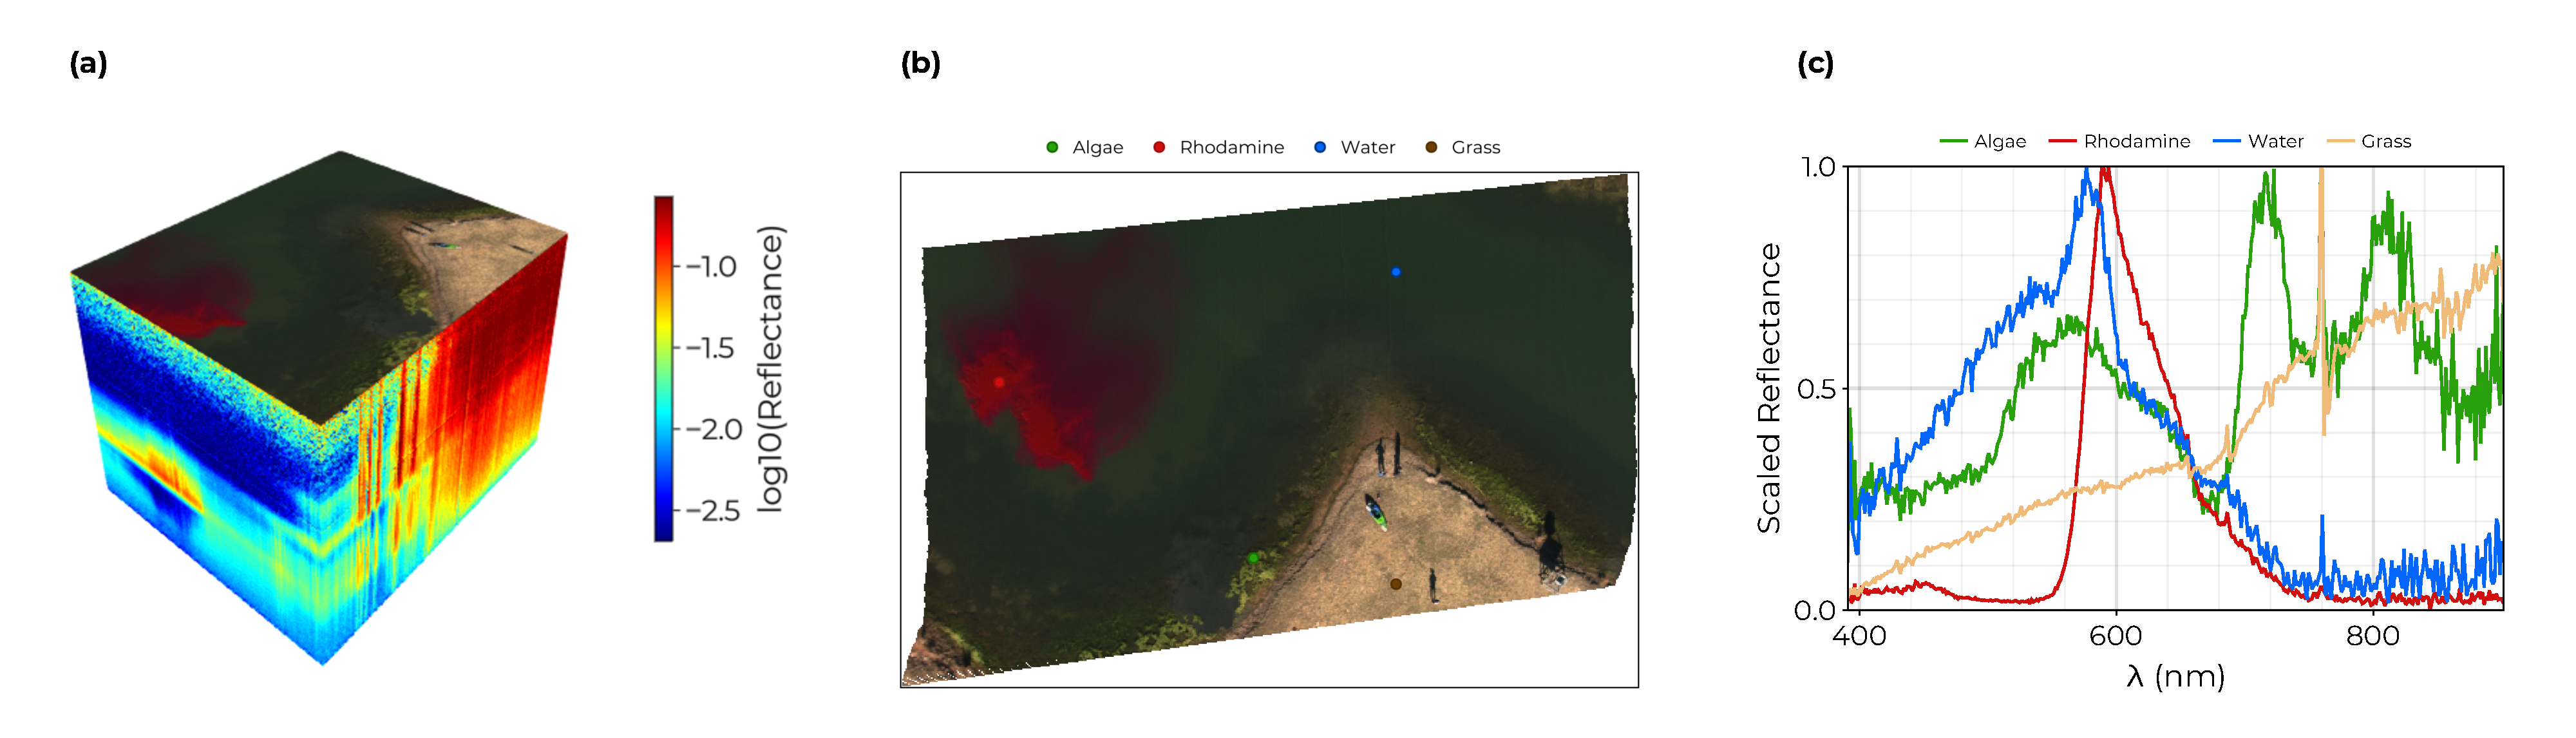
\includegraphics[width=15.5cm]{paper/figures/methods/sample-spectra.pdf}
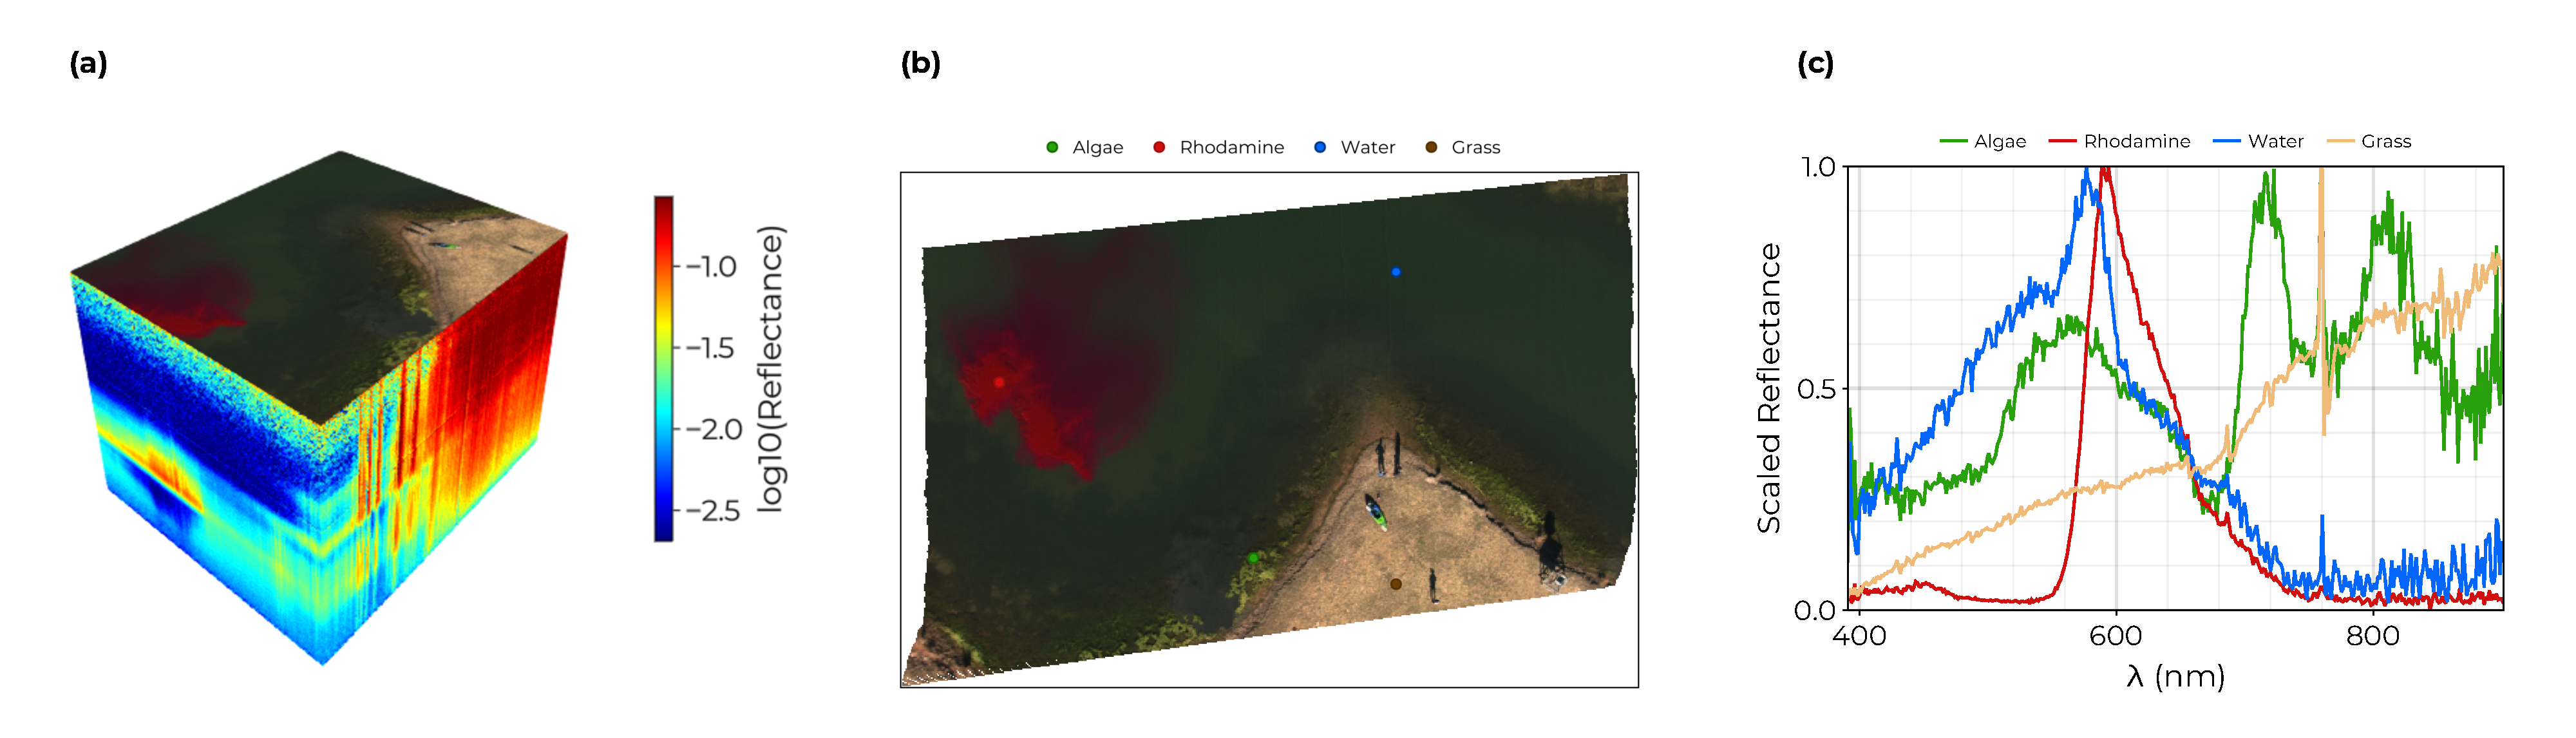
\includegraphics[width=\columnwidth]{paper/figures/methods/sample-spectra.pdf}
%\end{adjustwidth}
\caption{(\textbf{a}) Sample hyperspectral data cube. Spectra are plotted using their geographic position with the log10-reflectance colored along the z axis and a pseudo-color image on top. (\textbf{b}) Points taken from a sample hyperspectral data cube corresponding to algae, rhodamine dye, water, and dry grass. (\textbf{c}) Reflectance spectra for the exemplar points scaled so the peak value of each spectrum is $1.0$. (\textbf{d}) The location of the pond in Montague, Texas where data were collected for this study.\label{fig:sample-spectra}}
\end{figure}  


\subsection{Generative Topographic Mapping}

The Generative Topographic Mapping (GTM) is an unsupervised latent variable model developed by Bishop, Svens\'en, and Williams \cite{gtm-bishop-1}. The GTM takes inspiration from Kohonen's self-organizing map which enables an unsupervised classification of high dimensional data into a (typically) two-dimensional grid of nodes such that nodes near each near each other in the mapping space

- mention 

\begin{equation}\label{eq:latent-prob}
    p(\xi) = \frac{1}{K}\sum_k^K \delta(\xi - \xi_k)
\end{equation}

\begin{equation}\label{eq:data-prob}
    p\left( \mathbf{x} \mid \xi, W, \beta \right)  = \mathcal{N}(\psi,\, \beta^{-1})
\end{equation}

\begin{equation}\label{eq:psi}
    \psi = W\phi(\xi)
\end{equation}

Parameter prior (used for model weight regularization), i.e. assuming a Gaussian distribution with mean 0 for each weight where $\lVert \cdot \rVert_{F}$ is the Frobenius norm.
\begin{equation}\label{eq:weight-prior}
    p(W \mid \alpha) =  \left( \frac{\alpha}{2\pi} \right)^{MD/2}\exp\left(-\frac{\alpha}{2}\lVert W \rVert_{F}^2\right)
\end{equation}
\begin{equation}\label{eq:llh}
    \mathcal{L}(W, \beta) = \sum_n^N \ln \left(\dfrac{1}{K}\sum_k^K p(\mathbf{x}_n \mid \xi_k, W, \beta) \right)
\end{equation}

Expectation Maximization Algorithm:

Expectation step:
\begin{equation}\label{eq:responsibility}
    R_{kn} = p(\xi_k \mid \mathbf{x}_n, W, \beta) = \dfrac{p(\mathbf{x}_n \mid \xi_k, W, \beta)}{\sum\limits_{k'}^{K} p(\mathbf{x}_n \mid \xi_{k'}, W, \beta)}
\end{equation}

Maximization step:

Definition of the diagonal matrix, $G$, with entries
\begin{equation}
    G_{kk}  = \sum\limits_n^N R_{kn}
\end{equation}
and all others $0$.

\begin{equation}\label{eq:W-update}
    \left(\Phi^T G \Phi + \dfrac{\alpha}{\beta}I \right)W_{\text{new}} = \Phi^T R X 
\end{equation}

\begin{equation}
    \hat{\xi}_n = \sum_{k}^K R_{kn}\xi_k
\end{equation}

- GTM paper original \cite{gtm-bishop-1}
- GTM developments paper \cite{gtm-bishop-2}
- GTM code \cite{gtm-code}
- implementation designed to work in MLJ ecosystem \cite{blaom2020mlj}


at a pond in Montague, north Texas (shown in panel d of Fig~\ref{fig:sample-spectra})


\subsection{UAV-Based Hyperspectral Imaging}
A Freefly Alta-X autonomous quadcopter was used as a UAV platform for the robotic team.

The Alta-X is specifically designed to carry cameras and has a payload of up to 35 lbs. We equipped the UAV with a Resonon Pika XC2 visible+near-infrared (VNIR) hyperspectral imager. 

For each image pixel, this camera samples 462 wavelengths ranging from 391 to 1011 nm. 

Additionally, the UAV includes an upward facing Ocean Optics UV-Vis-NIR spectrometer with a cosine corrector to capture the incident downwelling irradiance spectrum.

Data collection by the hyperspectral imager is controlled by an attached Intel NUC small-form-factor computer. 

A second processing NUC is also included for onboard georectification and generation of data products.

The collected hyperspectral images (HSIs) are stored locally on a solid state drive that is simultaneously mounted by the processing computer.

- georetification \cite{muller2002program, baumker2001new, mostafa2000multi}

\subsection{Data Collection and Pre-Processing}
- Julia programming language used \cite{bezanson2012julia}



\subsection{Image Segmentation with the Normalized Spectral Similarity Score}


%%%%%%%%%%%%%%%%%%%%%%%%%%%%%%%%%%%%%%%%%%
\section{Results}

\subsection{GTM Fit}

\begin{figure}[t]
\centering
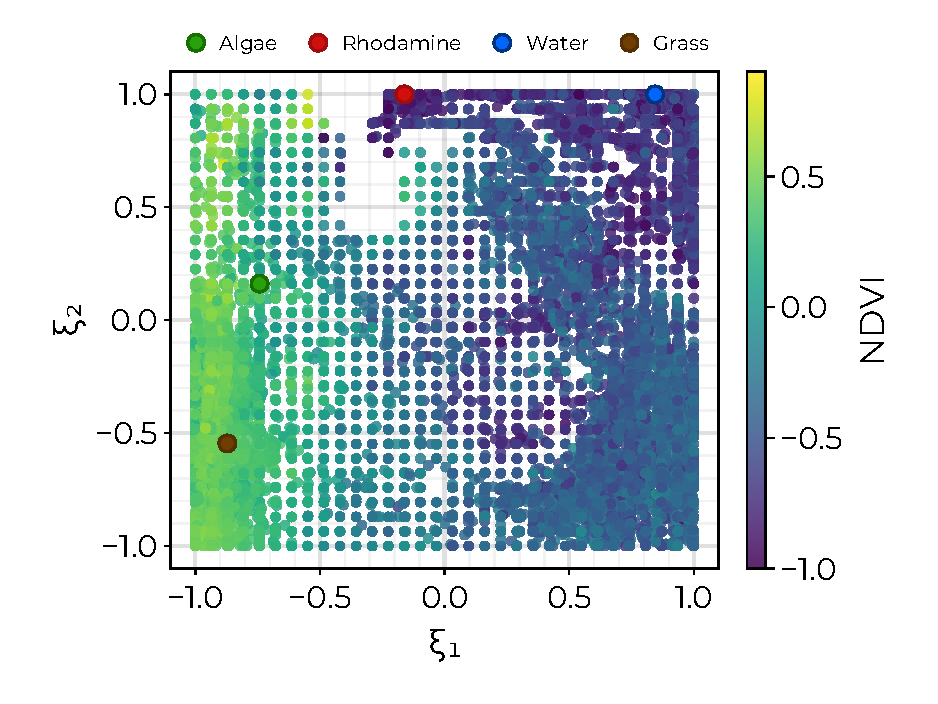
\includegraphics[width=0.8\columnwidth]{paper/figures/results/square-ndvi.pdf}
\caption{GTM Map: We plot the mean position of each data point in the latent space with points colored by the their associated NDVI values. The locations of the exemplar points for algae, rhodamine dye, water, and dry grass are shown in the latent space illustrating that the GTM has clearly distinguished land, near-land, and water pixels.\label{fig:}}
\end{figure}  


\subsection{Hyperparamter Optimization with BIC}


\begin{figure}[t]
%\begin{adjustwidth}{-\extralength}{0cm}
\centering
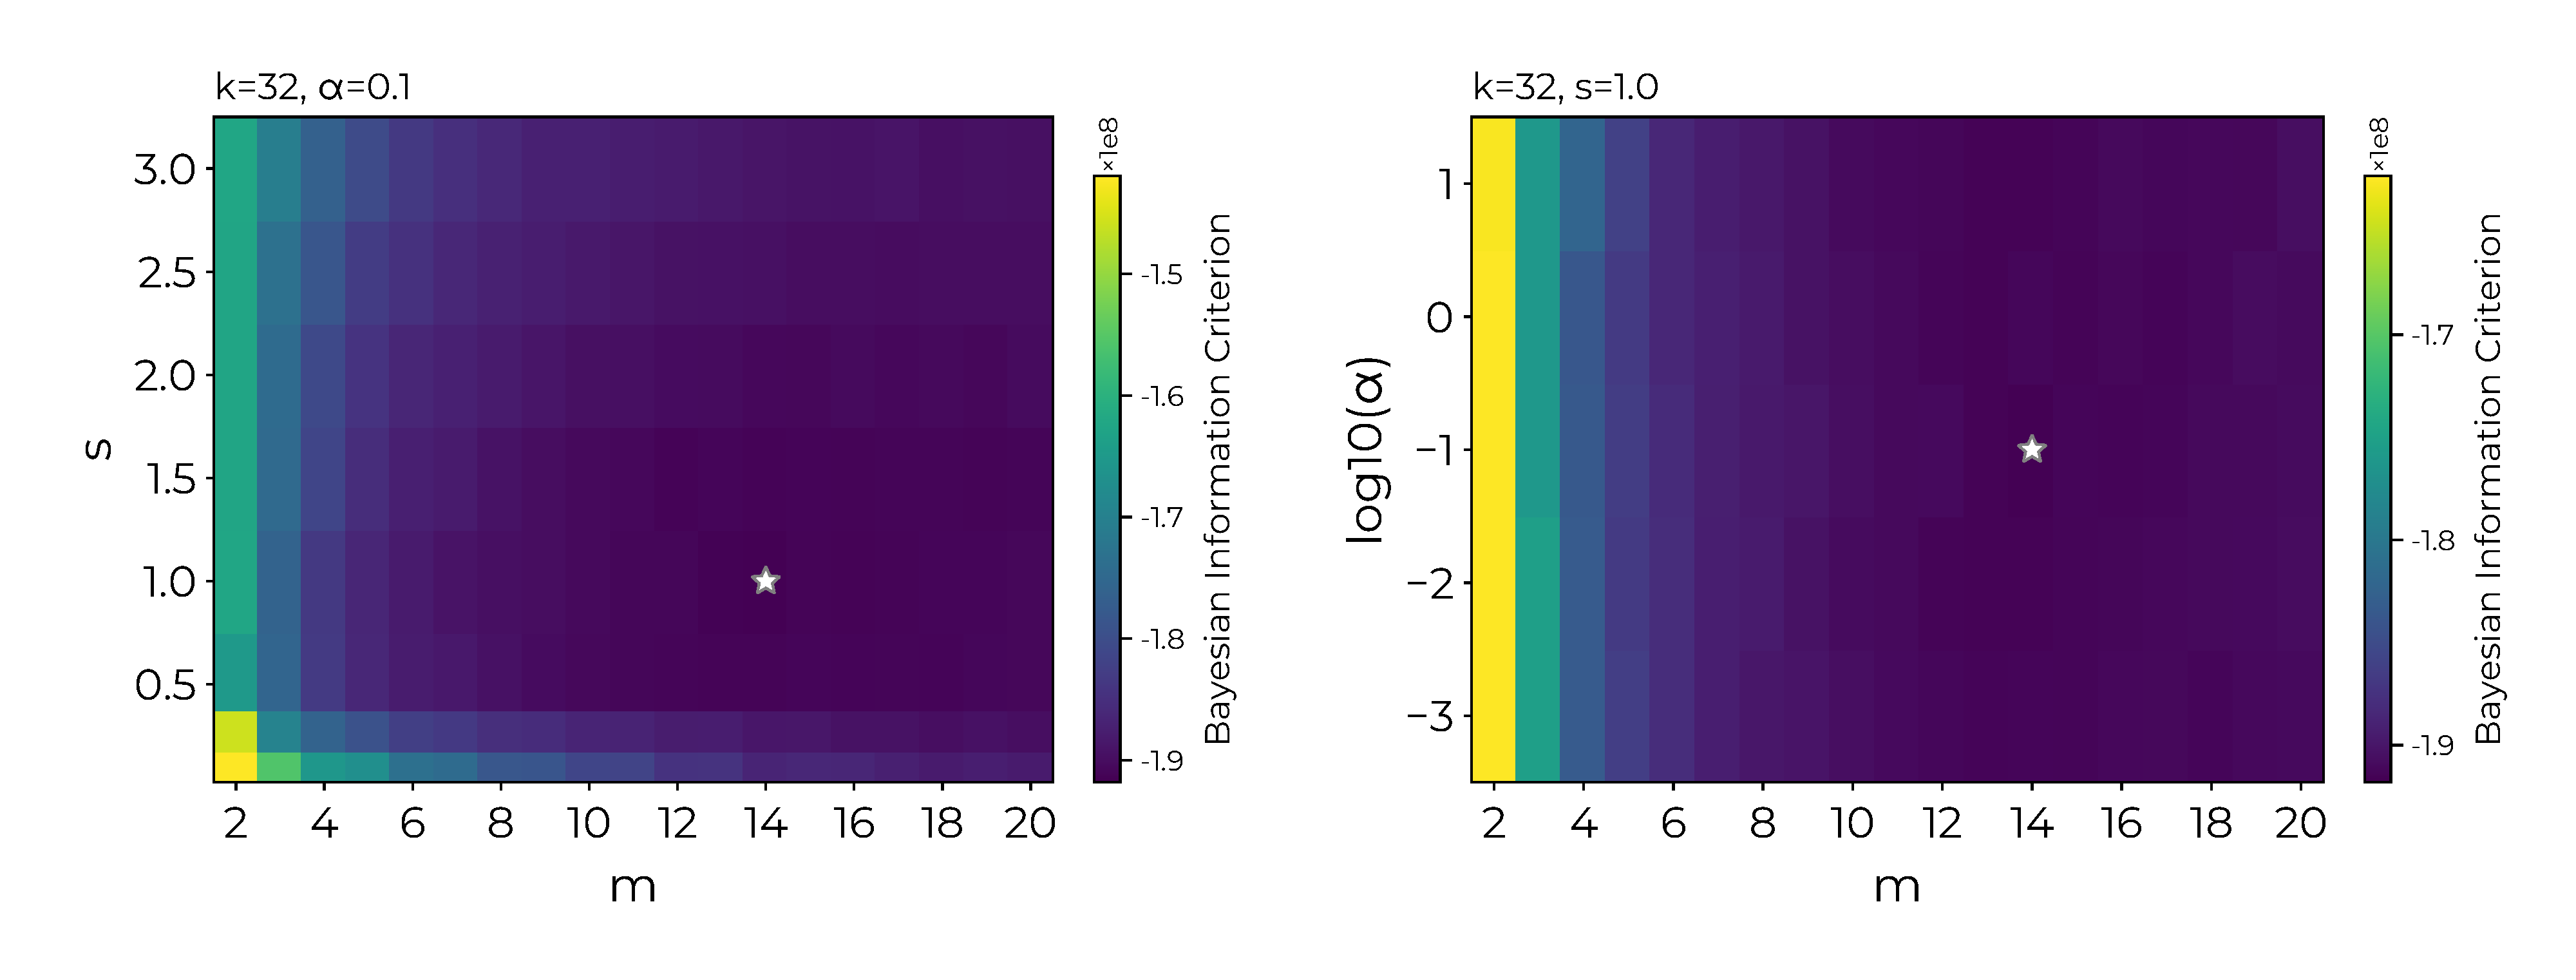
\includegraphics[width=\textwidth]{paper/figures/results/bic.pdf}
%\end{adjustwidth}
\caption{Results of the hyperparameter search. Left: Variation of BIC with $m$ and $s$ for fixed $\alpha=0.1$. Right: Variation of the BIC with with $m$ and $\alpha$ for fixed $s=1.0$. The white star in each plot indicates the parameters with the lowest BIC.\label{fig:hp-results}}
\end{figure}  


\subsection{Spectral Signatures}


\begin{figure}[t]
\begin{adjustwidth}{-\extralength}{0cm}
\centering
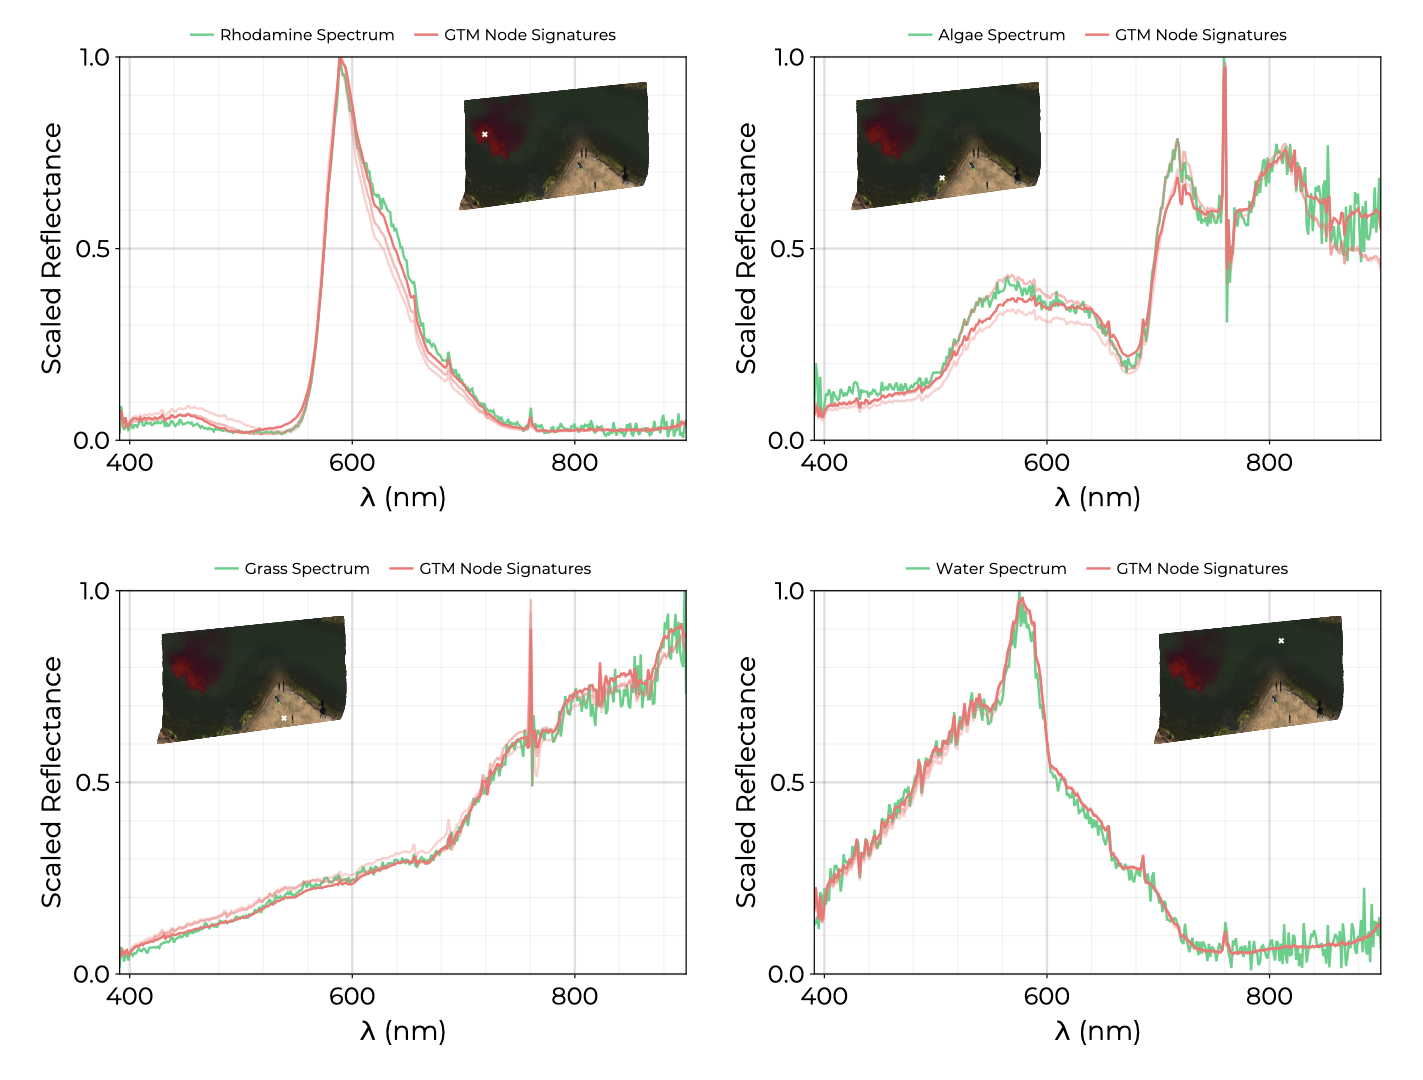
\includegraphics[width=15.5cm]{paper/figures/results/spectral-signatures.png}
\end{adjustwidth}
\caption{GTM Node Signatures corresponding to the exemplar spectra for the rhodamine plume (top left), algae (top right), dry grass (bottom left), and open water (bottom right). \label{fig:spectral-signautes}}
\end{figure}  

\subsection{Water Class Map}

\begin{figure}[t]
\begin{adjustwidth}{-\extralength}{0cm}
\centering
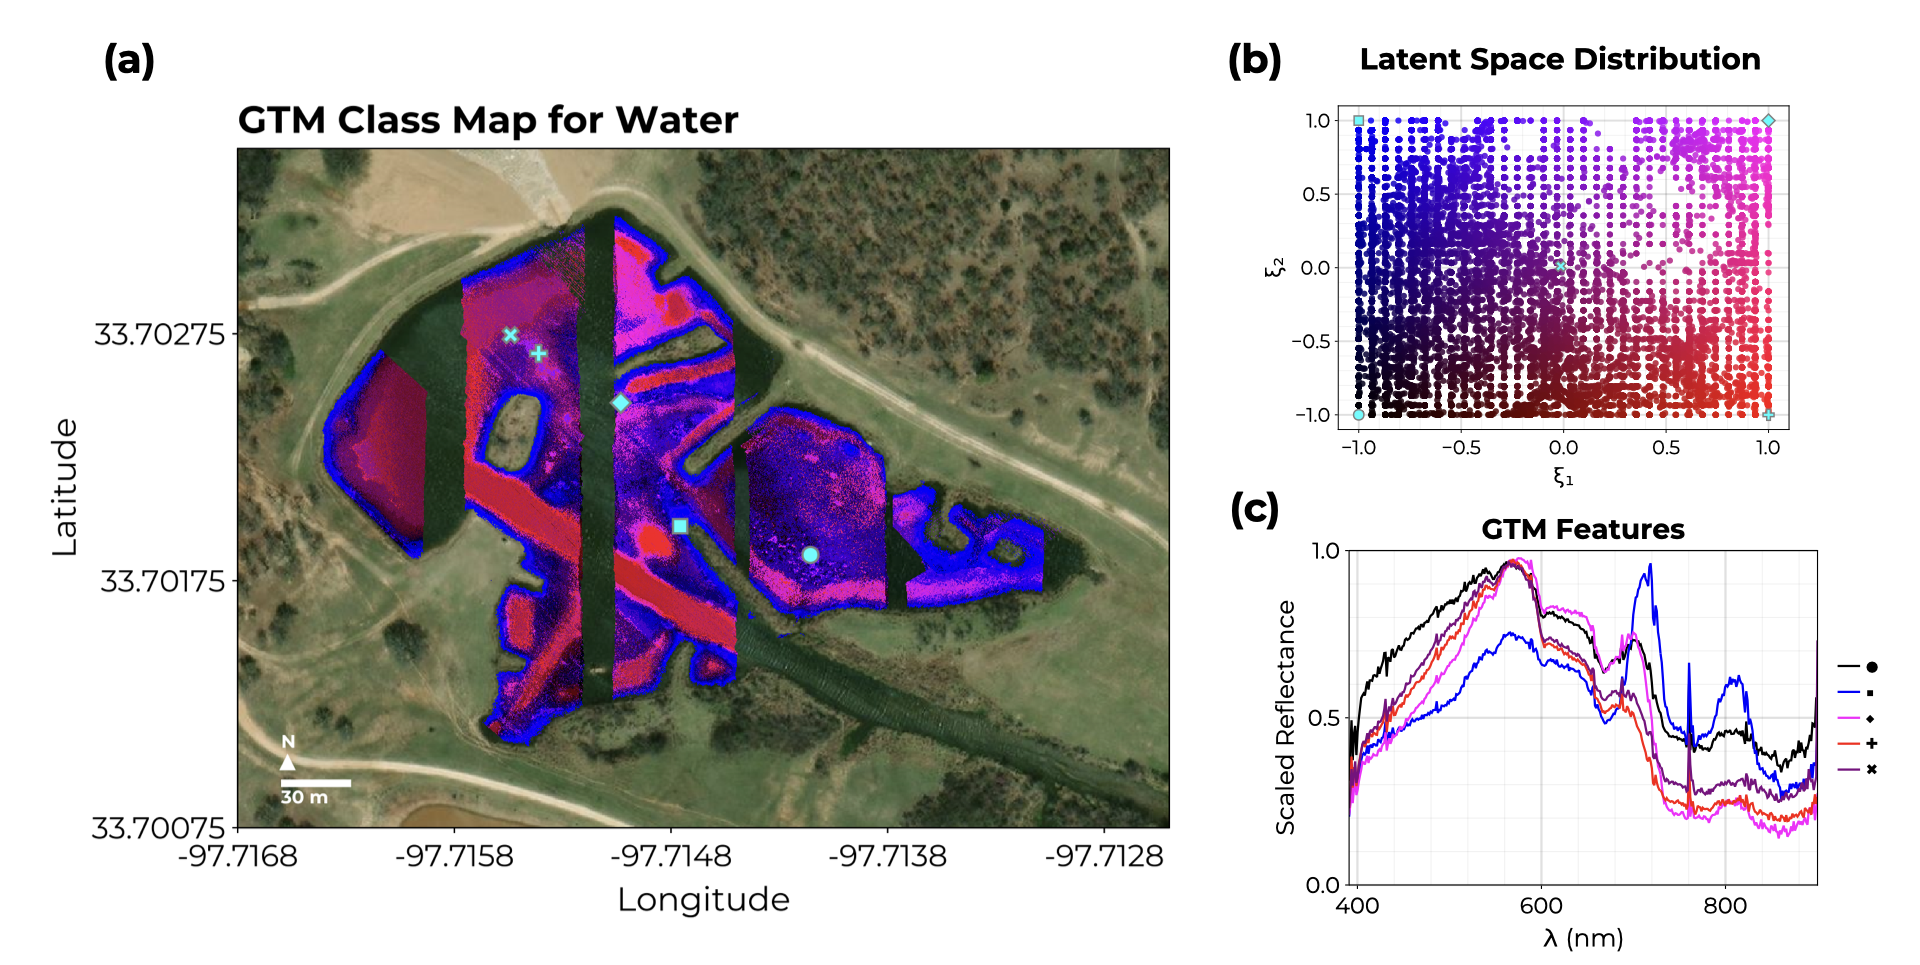
\includegraphics[width=18.0cm]{paper/figures/results/gtm-water.png}
\end{adjustwidth}
\caption{Classification map for GTM trained solely on water pixels (no land and no rhodamine plume). \textbf{(a)} GTM applied to all water pixels colored by their associated position in the latent space. \textbf{(b)} Representation of the poitns from the training set in the latent space. The points are colored with $\xi_1$ corresponding to red and $\xi_2$ corresponding to blue. \textbf{(c)} The associated GTM spectral signatures, $\Psi_i$, corresponding to the four corners and center of the GTM latent space. \label{fig:gtm-water}}
\end{figure}  


\subsection{Algae Identification}


\begin{figure}[t]
\begin{adjustwidth}{-\extralength}{0cm}
\centering
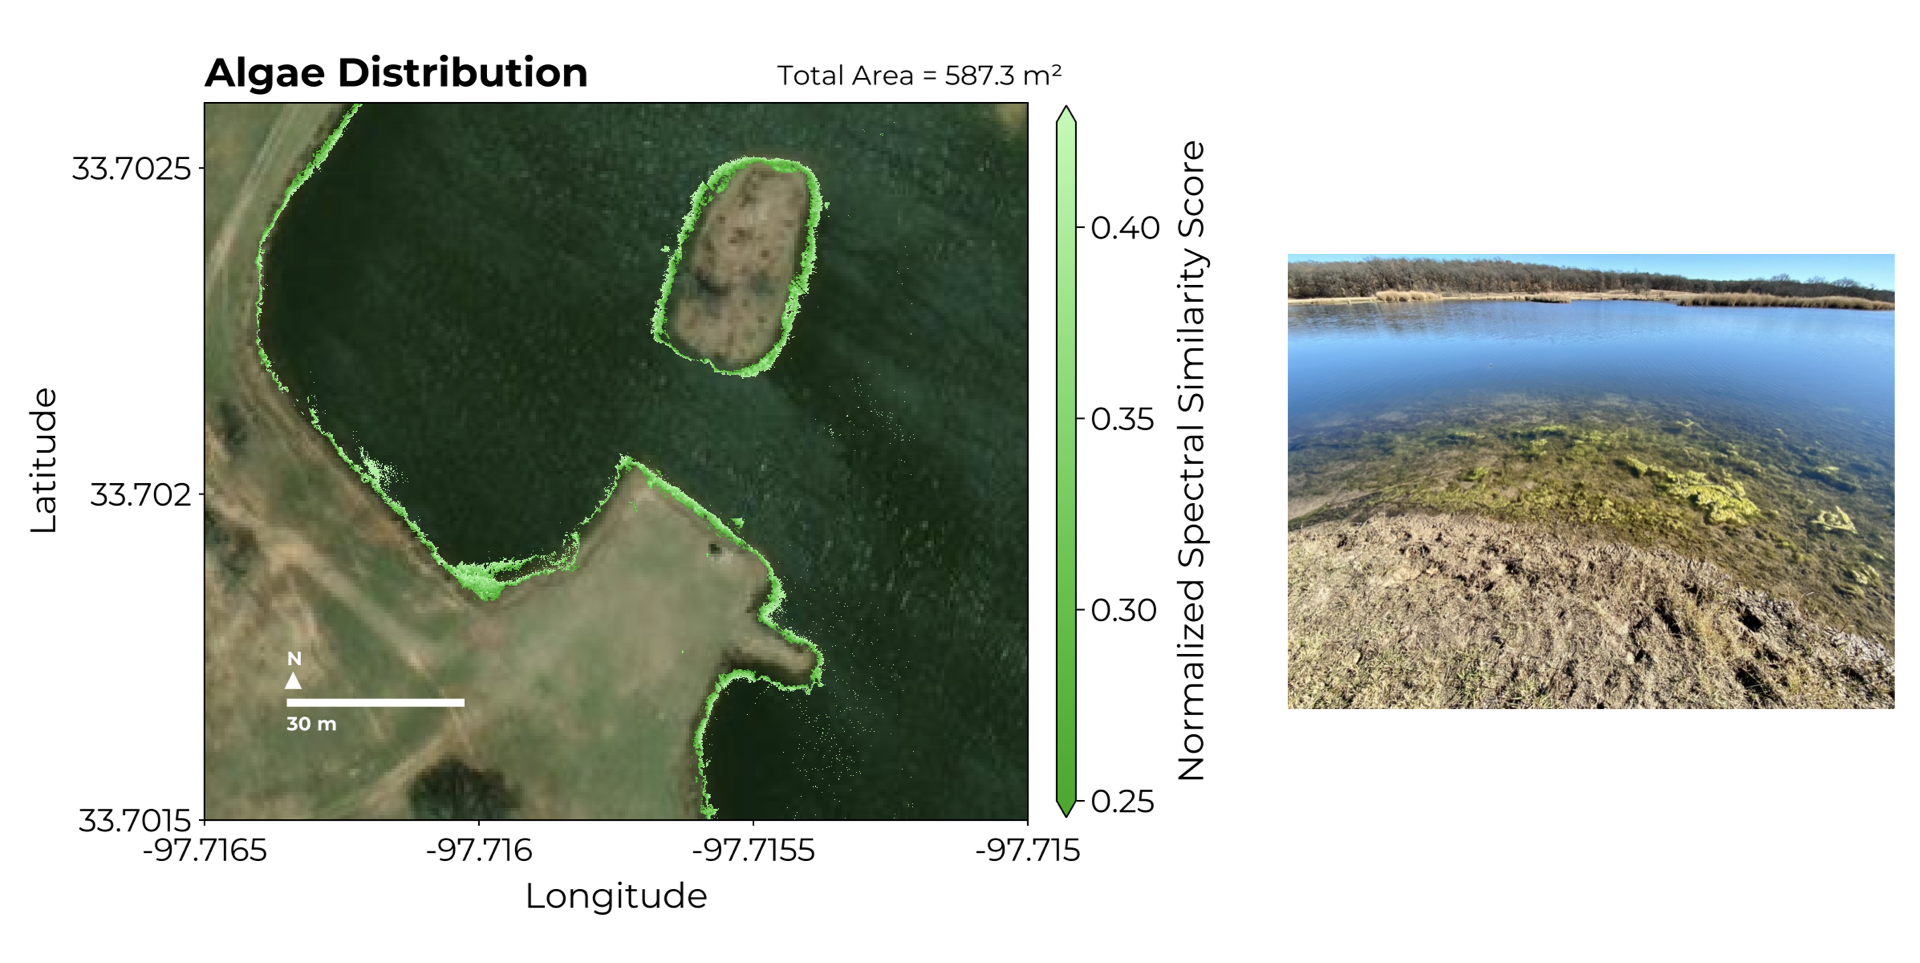
\includegraphics[width=15.5cm]{paper/figures/results/algae.png}
\end{adjustwidth}
\caption{\label{fig:algae-map}}
\end{figure}  



\subsection{Rhodamine Dye Plume Identification}

\begin{figure}[t]
\begin{adjustwidth}{-\extralength}{0cm}
\centering
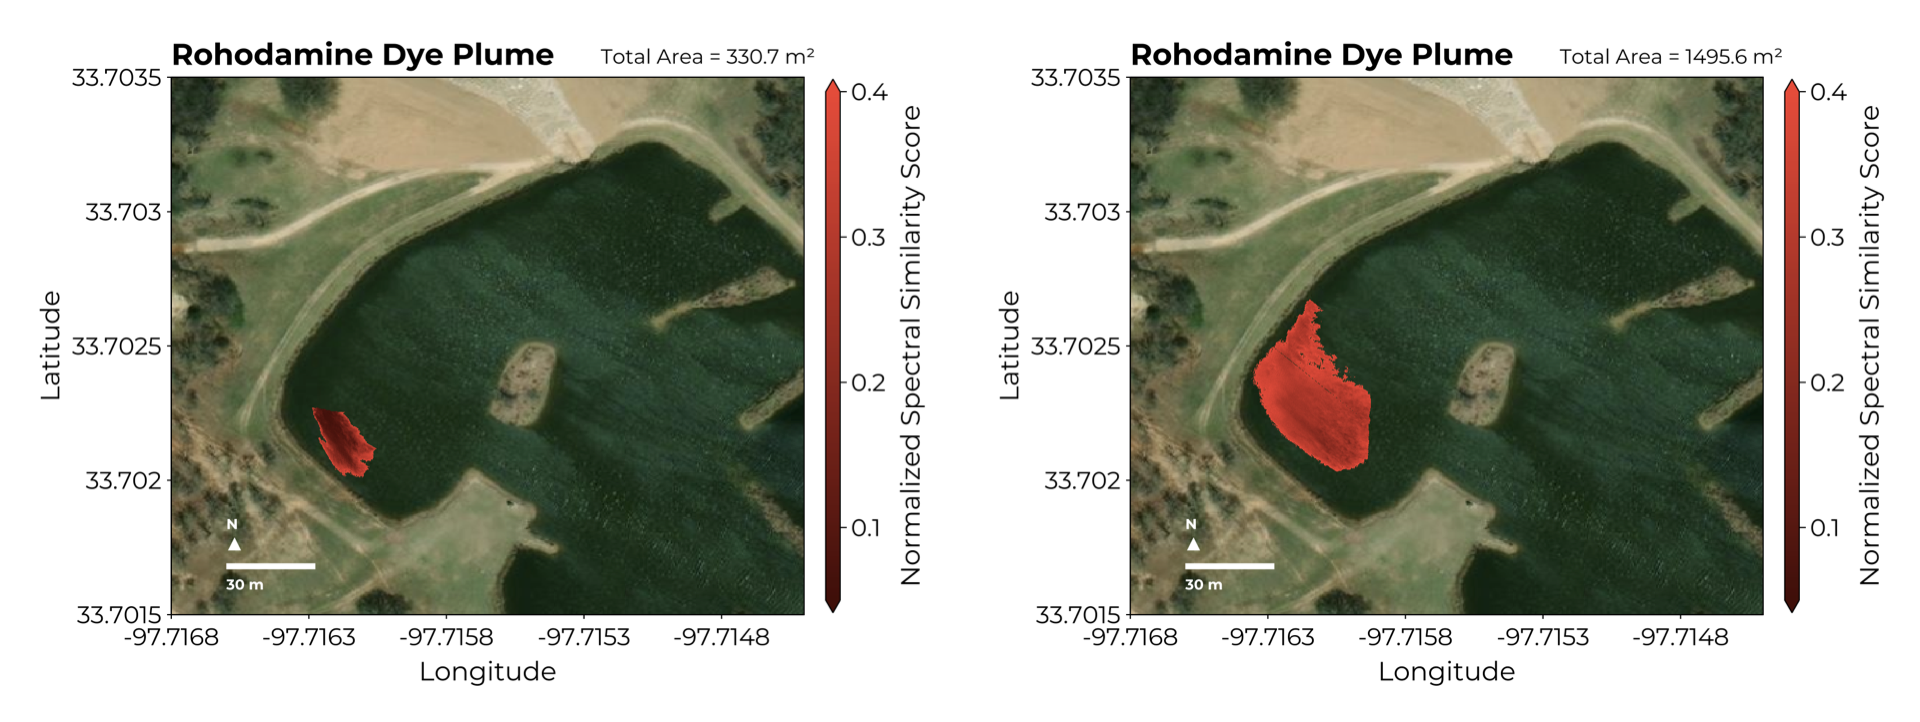
\includegraphics[width=15.5cm]{paper/figures/results/rhodamine.png}
\end{adjustwidth}
\caption{\label{fig:rhodamine-map}}
\end{figure}  




%%%%%%%%%%%%%%%%%%%%%%%%%%%%%%%%%%%%%%%%%%
\section{Discussion}

\subsection{Summary of GTM applications in our paper}
\subsection{Comparison to other existing approaches in literature}
- Is there much done for classification in real time? 
\subsection{Comparison to Spectral Unmixing}
- Here we can re-interpret the GTM model as performing a type of Bayesian spectral unmixing and suggest how the method could be further extended to work in this domain. Critically, other traditional methods work by observing that pure endmembers form the vertices of a simplex. 

\subsection{Other applications of GTM}
- Discuss use of GTM means/modes/responsibilities feature transformer for supervised models (e.g. better than PCA) 
- Use of GTM classes to aid autonomous data collection by identification of "interesting" regons


%%%%%%%%%%%%%%%%%%%%%%%%%%%%%%%%%%%%%%%%%%
\section{Conclusions}


%%%%%%%%%%%%%%%%%%%%%%%%%%%%%%%%%%%%%%%%%%
\vspace{6pt} 

%%%%%%%%%%%%%%%%%%%%%%%%%%%%%%%%%%%%%%%%%%
%% optional
%\supplementary{The following supporting information can be downloaded at:  \linksupplementary{s1}, Figure S1: title; Table S1: title; Video S1: title.}

% Only for journal Methods and Protocols:
% If you wish to submit a video article, please do so with any other supplementary material.
% \supplementary{The following supporting information can be downloaded at: \linksupplementary{s1}, Figure S1: title; Table S1: title; Video S1: title. A supporting video article is available at doi: link.}

% Only for journal Hardware:
% If you wish to submit a video article, please do so with any other supplementary material.
% \supplementary{The following supporting information can be downloaded at: \linksupplementary{s1}, Figure S1: title; Table S1: title; Video S1: title.\vspace{6pt}\\
%\begin{tabularx}{\textwidth}{lll}
%\toprule
%\textbf{Name} & \textbf{Type} & \textbf{Description} \\
%\midrule
%S1 & Python script (.py) & Script of python source code used in XX \\
%S2 & Text (.txt) & Script of modelling code used to make Figure X \\
%S3 & Text (.txt) & Raw data from experiment X \\
%S4 & Video (.mp4) & Video demonstrating the hardware in use \\
%... & ... & ... \\
%\bottomrule
%\end{tabularx}
%}

%%%%%%%%%%%%%%%%%%%%%%%%%%%%%%%%%%%%%%%%%%
\authorcontributions{FIXME}

\funding{FIXME}

\institutionalreview{Not applicable}

\informedconsent{Not applicable}

\dataavailability{We encourage all authors of articles published in MDPI journals to share their research data. In this section, please provide details regarding where data supporting reported results can be found, including links to publicly archived datasets analyzed or generated during the study. Where no new data were created, or where data is unavailable due to privacy or ethical restrictions, a statement is still required. Suggested Data Availability Statements are available in section ``MDPI Research Data Policies'' at \url{https://www.mdpi.com/ethics}.} 


\acknowledgments{In this section you can acknowledge any support given which is not covered by the author contribution or funding sections. This may include administrative and technical support, or donations in kind (e.g., materials used for experiments).}

\conflictsofinterest{Declare conflicts of interest or state ``The authors declare no conflicts of interest.'' Authors must identify and declare any personal circumstances or interest that may be perceived as inappropriately influencing the representation or interpretation of reported research results. Any role of the funders in the design of the study; in the collection, analyses or interpretation of data; in the writing of the manuscript; or in the decision to publish the results must be declared in this section. If there is no role, please state ``The funders had no role in the design of the study; in the collection, analyses, or interpretation of data; in the writing of the manuscript; or in the decision to publish the results''.} 

%%%%%%%%%%%%%%%%%%%%%%%%%%%%%%%%%%%%%%%%%%
%% Optional

%% Only for journal Encyclopedia
%\entrylink{The Link to this entry published on the encyclopedia platform.}

\abbreviations{Abbreviations}{
The following abbreviations are used in this manuscript:\\

\noindent 
\begin{tabular}{@{}ll}
UAV & Unmanned Aerial Vehicle \\
SOM & Self Organizing Map \\ 
GTM & Generative Topographic Mapping  \\
HSI & Hyperspectral Image \\ 
CDOM & Colored Dissolved Organic Matter \\
HAB & Harmful Algal Bloom 
\end{tabular}
}

%%%%%%%%%%%%%%%%%%%%%%%%%%%%%%%%%%%%%%%%%%
%% Optional
\appendixtitles{yes} % Leave argument "no" if all appendix headings stay EMPTY (then no dot is printed after "Appendix A"). If the appendix sections contain a heading then change the argument to "yes".
\appendixstart
\appendix
\section[\appendixname~\thesection]{Hyperparameter Search Results}

\begin{table}[H]
  \caption{The top 25 models from the hyperparameter search. A variety of GTM were trained to explore the the impact of varying m, $\alpha$, and s.\label{tab:hp-search}}
  \begin{adjustwidth}{-\extralength}{0cm}
  \newcolumntype{C}{>{\centering\arraybackslash}X}
  \begin{tabularx}{\fulllength}{CCCCCC}
    \toprule
    \textbf{m} & \textbf{$\alpha$} & \textbf{s} & \textbf{k} & \textbf{BIC} & \textbf{AIC} \\
    \midrule
    14 & 0.1 & 1.0 & 32 & \textbf{-1.918e8} & -1.926e8\\
    13 & 0.01 & 1.0 & 32 & -1.917e8 & -1.923e8\\
    16 & 0.01 & 1.5 & 32 & -1.917e8 & -1.926e8\\
    14 & 10.0 & 1.0 & 32 & -1.917e8 & -1.924e8\\
    16 & 0.001 & 1.5 & 32 & -1.917e8 & -1.926e8\\
    13 & 1.0 & 1.0 & 32 & -1.917e8 & -1.923e8\\
    13 & 10.0 & 1.0 & 32 & -1.917e8 & -1.923e8\\
    14 & 0.001 & 1.5 & 32 & -1.916e8 & -1.924e8\\
    13 & 0.1 & 1.0 & 32 & -1.916e8 & -1.923e8\\
    14 & 0.01 & 1.0 & 32 & -1.916e8 & -1.924e8\\
    15 & 0.01 & 1.5 & 32 & -1.916e8 & -1.925e8\\
    14 & 0.01 & 1.5 & 32 & -1.916e8 & -1.923e8\\
    15 & 1.0 & 1.0 & 32 & -1.916e8 & -1.924e8\\
    18 & 0.01 & 1.5 & 32 & -1.916e8 & -1.928e8\\
    12 & 0.01 & 1.0 & 32 & -1.916e8 & -1.921e8\\
    15 & 0.01 & 0.5 & 32 & -1.915e8 & -1.924e8\\
    17 & 1.0 & 1.0 & 32 & -1.915e8 & -1.926e8\\
    16 & 0.1 & 1.0 & 32 & -1.915e8 & -1.925e8\\
    18 & 0.001 & 1.5 & 32 & -1.915e8 & -1.928e8\\
    13 & 0.001 & 1.0 & 32 & -1.915e8 & -1.922e8\\
    12 & 1.0 & 1.0 & 32 & -1.915e8 & -1.921e8\\
    17 & 0.001 & 1.5 & 32 & -1.915e8 & -1.926e8\\
    15 & 0.001 & 1.5 & 32 & -1.915e8 & -1.923e8\\
    15 & 10.0 & 1.0 & 32 & -1.915e8 & -1.923e8\\
    12 & 0.1 & 1.5 & 32 & -1.915e8 & -1.92e8\\
    \bottomrule
  \end{tabularx}
  \end{adjustwidth}
\end{table}


%%%%%%%%%%%%%%%%%%%%%%%%%%%%%%%%%%%%%%%%%%
\begin{adjustwidth}{-\extralength}{0cm}
%\printendnotes[custom] % Un-comment to print a list of endnotes

\reftitle{References}

%=====================================
% References, variant A: external bibliography
%=====================================
\bibliography{paper/references.bib}

%%%%%%%%%%%%%%%%%%%%%%%%%%%%%%%%%%%%%%%%%%
\PublishersNote{}
\end{adjustwidth}
\end{document}

